
\chapter{Introduction}
\section{The Standard Model of Particle Physics}
Particle physics deals with the fundamental matter particles and the interactions between them. It also explains their properties such as mass, spin and charge. 
\subsection{The Fundamental Particles}
In particle physics an elementary particle or fundamental particle is the one that has no internal structure or is not made of other particles. The current fundamental particles are called fermions which are called matter particles and other type are called anti-matter particles and bosons, which are the force carrying particles and allow interactions between matter particles.
\subsubsection{Fermions}
In Standard Model~(SM) there are two types of fermions, the quarks and the leptons. The fermions obey the Pauli Exclusion Principle which states that two fermions can not have same state at the same time~i.e.~two fermions can not have same quantum numbers. All fermions have half integral spin. In SM there are twelve fermions which are divided into six generations, each one  has two particles. Fermions are divided into two groups,~leptons and quarks. The leptons have elementary charge of $-1$. Leptons have three flavors of charged particle, electron~$e$, muon~$\mu$ and tau~$\tau$, each lepton has corresponding neutral particle called neutrino. Electron is the only lepton which is stable in the universe from these six leptons. All the other leptons are massive and not stable hence decay into other stable particles.

Quarks have three generations and each one has two types. These six quarks are up~(u), down~(d), strange~(s), charm~(c), bottom~(b) and top~(t). The up~(u) and down~(d) quarks are only stable. The other quarks are very unstable and decay very quickly. Quarks interact with each other by the exchange of particles called gluon. Quarks are the particles which make hadrons~(baryons and mesons).
These twelve fermions have corresponding anti particles called anti-fermions. Electron's antiparticle is positron having same mass but opposite charge of +1, and muon's anti particle is anti muon with charge +1, similarly is the case for all other fermions. Anti-fermion has same mass as that of the corresponding fermion but opposite charge. 

\begin{figure}[h]
\centering
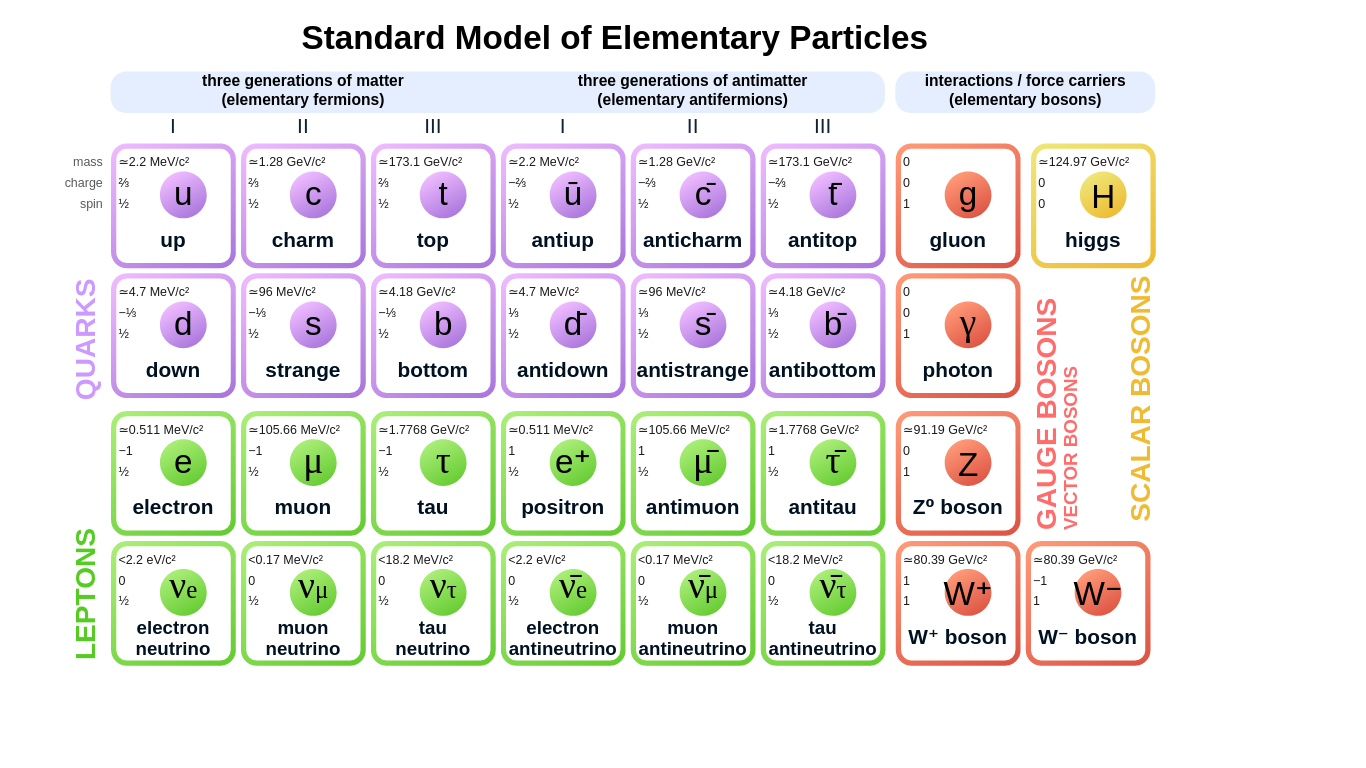
\includegraphics[scale=0.35]{chapter1/sm.png} 
\centering
\caption{Fermions and Bosons in the Standard Model,~figure adopted from~\cite{enwiki:1045150258}.}
\label{Fermions}
\end{figure}

\subsubsection{Bosons}
In standard model, vector bosons~(photons, gluons, graviton, $W$ and $Z$ boson) have integer spin~(spin=1,2) and scaler boson~(Higgs) has no spin~(spin=0). The vector bosons are mediator of interactions~(force) between elementary particles and scaler boson gives mass to other elementary particles. Boson are different from fermions as they obey Bose-Einstein distribution whereas fermions obey Fermi-Dirac distribution. Boson can exist in both states either elementary, like photons, gluons or in a combined state, like mesons.  
\subsubsection{Gluons}
Gluons mediate the strong interaction, which is responsible for the formation of hadrons. The hadrons are of two types, baryons and mesons. Baryon is composed of three quarks and meson has two quarks~(quark-antiquark)  state. Protons and neutrons are baryons, formed by the gluons and form atomic nucleus. Like quarks, gluons have a color and an anti color charge.
\subsubsection{Electroweak Bosons}
Weak bosons are of three types: $W^{+},W^{-},Z^{0}$. These bosons are the mediators of weak interaction. Unlike other bosons these are quite massive. The photon, which is a massless and charge less stable particle, which mediates the electromagnetic interaction. These four bosons are responsible for electroweak~(combined electromagnetic and weak) interaction between fundamental particles.
\subsubsection{Higgs boson}
In the Standard Model, the only massive scalar boson with zero spin is the Higgs boson,~an unstable particle with zero electric charge and no colour charge. Higgs boson decays into other particles almost immediately after it's production. The Higgs boson are the quanta of field called Higgs field which gives mass to elementary particles via mechanism called Higgs mechanism.
\begin{figure}
\centering
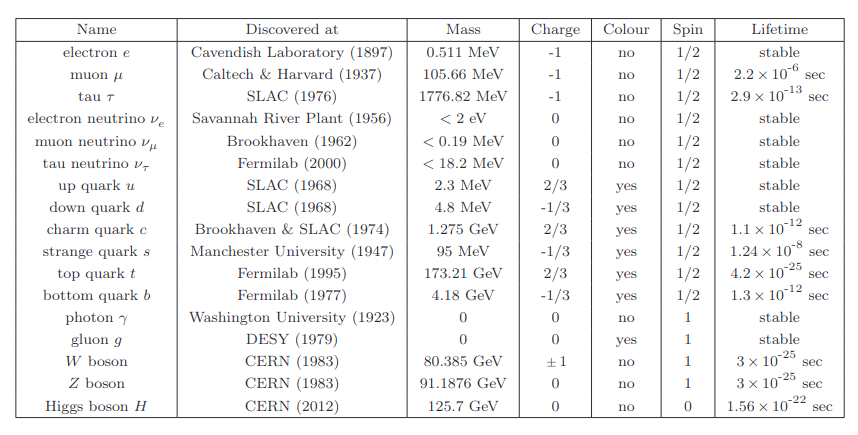
\includegraphics[scale=0.4]{chapter1/particle-sm.png}
\caption{Known Elementary particles in Standard Model. Parameters are taken from ~\cite{ParticleDataGroup:2016lqr}.}
\end{figure}
\section{Beyond Standard Model}
The theoretical predictions that try to explain the shortcomings in SM are referred to as Physics Beyond Standard Model~(BSM). The SM successfully explains particle physics phenomenology in~$\approx$ TeV scale. There are six major question in SM~\cite{Clarke:2016vnr}:
\begin{itemize}
\item Higgs Sector~(What is the nature of electro-weak symmetry breaking?)
\item Naturalness~(Is the mass of Higgs natural?)
\item Neutrino mass~(What is the mechanism by which neutrinos gain mass?)
\item Baryon Asymmetry of the Universe~(How the Universe has more baryons than anti baryons?)
\item Strong CP Problem~(Small neutron electric dipole moment?)
\item Dark Matter~(what is the nature of non-luminous but gravitationally interacting matter?)
\end{itemize}
\subsection{Grand Unification}
The Grand Unification theory~(GUT) predicts that electromagnetic, strong and weak force can merge into a single force at very high energy scale. According to Grand Unified Theory we can merge all three fundamental forces into single one called electro nuclear force. Such unified force can be broken into three fundamental forces by a Higgs like mechanism.  Grand unification models are expected at very high energy scale of about~$\approx 10^{16}~{GeV}$.
\subsection{Supersymmetry~(SUSY)}
Supersymmetry~\cite{article} predicts that each particle in SM either fermion or boson has a partner particle called superpartner. This can help us to explain why particles have mass. Symmetries are very important in modern physics, since they give a nice way to construct Lagrangian for a field or particle from which equation of motion can be found. Well-known examples of symmetries are symmetry under Lorentz transformation, translational symmetry in space-time as well as symmetry under isospin transformations. Supersymmetry is different from these symmetries in that it is invariant under transformation of bosonic field/particle to fermionic field/particle and vice versa. Supersymmetry combines fermionic field and bosonic field in a single field called a super field.\\
There are two class of particles in SM, fermions or bosons based on their spin. All Fermions have $1/2$ units of spin, while the bosons have integer spin~i.e. 0, 1, 2. According to Supersymmetry theory each particle in SM has a partner particle whose spin differs from the particle in integer multiple of 1/2. In this manner Supersymmetry brings two types of SM particles fermions and bosons together.
\subsection{String Theory}
According to String Theory the sub-atomic particles are like a vibrating one dimensional strings rather zero dimensional point particles. The mode of vibration of the string corresponds to the mass, charge and other properties of particle. These strings exist in an eleven dimensional or twelve dimensional universe. These strings can vibrate with different frequencies. These frequencies are responsible for the strings mass, charge and spin. A string can have many shapes, open like a line or closed like a circle or more complicated shapes.
\section{Elementary Particles Dynamics}
There are four fundamental forces in nature through which matter particles interacts with each other. These forces are carried by particles called mediators of force. On the basis of mediating particles these interactions are divided into several types, each one explained below, briefly.


\subsection{Quantum Electrodynamics}
In Quantum Electrodynamics~(QED) the electrically charged particles interact with each other by exchange of fields known as photon.\\
\begin{center}
\feynmandiagram [vertical=a to b] {
i1 [particle=\(e^{-}\)] -- [fermion] a -- [fermion] i2 [particle=\(e^{-}\)],
a -- [photon, edge label=\(q\)] b,
f1 [particle=\(e^{+}\)] -- [fermion] b -- [fermion] f2 [particle=\(e^{+}\)],
};
\end{center}

In above figure time flows horizontally, an electron and positron scattering mediated by a photon is shown. The anti-particle line is always directed backward in time while the particle is going forward. Pair production, Compton scattering and pair annihilation are the fundamental QED processes.  In quantum electrodynamics the force mediators could be photons, electrons or positrons. According the Feynman rule, momentum is conserved at each vertex of Feynman diagram and for the whole process also. \\
\begin{center}
\feynmandiagram [vertical=a to b] {
i1 [particle=\(e^{-}\)] -- [fermion] a -- [anti fermion] i2 [particle=\(e^{+}\)],
a -- [photon, edge label=\(\gamma\), momentum'=\(k\)] b,
f1 [particle=\(\mu^{+}\)] -- [fermion] b -- [anti fermion] f2 [particle=\(\mu^{-}\)],
};\\

\feynmandiagram [horizontal=a to b] {
i1 [particle=\(e^{-}\)] -- [fermion, very thick] a -- [fermion, opacity=0.2] i2 [particle=\(e^{+}\)],
a -- [red, fermion,  momentum'={[arrow style=red]\(k\)}] b,
f1 [particle=\(\gamma\)] -- [boson, opacity=0.2] b -- [boson, very thick] f2 [particle=\(\gamma\)],
};
\end{center}
\subsection{Quantum Chromodynamics}
Quantum chromodynamics is the theory of strong interaction between quarks and gluons, these are the fundamental particle that make up composite particles like hadrons.

Quarks have color charge and can be one of the three color charges red, blue, green. For any fundamental QCD process $q\rightarrow g+q$ the color charge of the quark can change but the flavour remains same. For example in a QCD interaction the color of up~(u) quark may change but its flavour does not change. The color charge is always conserved in any QCD interaction.
In the following Feynman diagram gluon must carry a unit of green and anti blue color charge to ensure color conservation.\\
\begin{center}
\feynmandiagram [horizontal=a to b] {
i1 [particle=\(q(g)\)] -- [fermion] a -- [fermion] i2 [particle=\(q(b)\)],
a -- [gluon, edge label=\(g\bar{b}\)] b,
f1 [particle=\(q(g)\)] -- [anti fermion] b -- [anti fermion] f2 [particle=\(q(b)\)],
};
\end{center}
Gluons have color charge unlike photons which are electrically neutral, thus the gluons can interact with other gluons.\\
The coupling constant for QCD is different from the QED. In QED at each vertex we need a factor of $\alpha$ = 1/137, because this number is very small thus we only need to consider Feynman diagrams with a small number of vertices. QCD coupling constant $\alpha_{s}$ depends upon the separation distance of the interacting particles~(we call it a running coupling constant) at very small distance the value of strong coupling constant become very small, this phenomenon in known as asymptotic freedom. Thus quarks and anti-quarks inside the proton wander like free particles, such behavior was found experimentally in deep inelastic scattering experiments~(DIS). Asymptotic freedom becomes more important in perturbation QCD theory.
\subsection{Weak Interaction}
All quarks and all leptons interact through weak force (leptons have no color charge hence can not interact though strong interaction; neutrinos are charge less, so they cannot interact through electromagnetic forces; but all quarks and leptons can interact through weak interactions.) There are two types of weak interactions: charged weak interactions which are mediated by $W$ boson and weak neutral interactions mediated by neutral $Z$ boson.\\

\begin{center}
\feynmandiagram [horizontal=a to b] {
i1 [particle=\(e^{-}\)] -- [fermion] a -- [fermion] i2 [particle=\(e^{-}\)],
a -- [boson, edge label=\(Z\)] b,
f1 [particle=\(\nu^{\mu}\)] -- [anti fermion] b -- [anti fermion] f2 [particle=\(\nu^{\mu}\)],
};\\

\feynmandiagram [horizontal=a to b] {
  a [particle=\(\mu^{-}\)] -- [fermion] b -- [fermion] f1 [particle=\(\nu_{\mu}\)],
  b -- [boson, edge label=\(W^{-}\)] c,
  f2 [particle=\(e^{-}\)] -- [anti fermion] c -- [fermion] f3 [particle=\(\nu_{e}\)],
};
\end{center}
The interactions in which the mediator is a $Z$ boson is known as neutral weak interaction.\\
The strong, electromagnetic and neutral weak interaction all share the feature that the same quark or lepton comes out when interaction occurs by an exchange of gluon, photon or $Z$ boson. In QCD the color of the quark may change but flavour of particle does not. The charged weak interactions are the only interactions that change flavor of the particles and in this sense they are the only ones capable of causing a true decay.

\begin{center}

\feynmandiagram [vertical=a to b] {
i1 [particle=\(\mu^{-}\)] -- [fermion] a -- [fermion] i2 [particle=\(\nu_{\mu}\)],
a -- [boson, edge label=\(W^{-}\)] b,
f1 [particle=\(\nu_{e}\)] -- [ fermion] b -- [fermion] f2 [particle=\(e^{-}\)],
};
\end{center}

Above Feynman diagram shows weak interaction of leptons in which a negative lepton~($e^{-}, \mu^{-},~\tau^{-}$) converts into the corresponding neutrino mediated by $W^{-}$ boson, $l^{-}\rightarrow\nu_{l}+W^{-}$.
Note in case of weak interaction of leptons, it can only convert into same generation i.e.~$e^{-}$ converts to $\nu_{e},$ and $\mu^{-}\rightarrow\mu^{-}$ with the emission or absorption of $W's$ boson, but $e^{-}$ never convert
into $\mu^{-}$ nor $\mu^{-}$ to $\nu_{e}$. Thus electroweak theory conserves the electron number, muon number, and tau number.

\begin{center}
\feynmandiagram [horizontal=a to b] {
i1 [particle=\(d\)] -- [fermion] a -- [fermion] i2 [particle=\(u\)],
a -- [boson, edge label=\(W^{-}\)] b,
f1 [particle=\(e\)] -- [anti fermion] b -- [fermion] f2 [particle=\(\nu_{e}\)],
};
\end{center}
If a quark interacts with $W^{+}$ boson it will convert into an other quark of same generation~i.e d-quark with charge -1/3 will convert into a u-quark of charge 2/3, similarly for other quarks. In such interactions the flavor of quark changes but color remain same. $W$ and $Z$ bosons also known as Intermediate vector bosons or weak bosons are the mediator of Weak Interactions. They are also called vector bosons due to their spin~(s=1). $W$ bosons have charge $\pm1$ and Z boson is electrically neutral. $W^{+}$ and $W^{-}$ are anti-particles of eachother and $Z$ boson is its own anti-particle. The life time of these bosons is very small with a half-life of about $3\times10^{-25}sec$.  

The $W$ boson is the only one which can cause nuclear transmutation by emission or absorption of leptons. The interaction with the exchange of $Z$ boson is similar to the interactions in QED. $Z$ boson can only transfer momentum or spin between interacting particles. In interaction with exchange of $Z$ boson electrically charged particles can not be emit or absorbed.

The $W$ and $Z$ boson are massive elementary particles with masses $80.4~GeV$~\cite{ddd77f409a1d4f53a9ea8bbf3f2e016d} and $91.2~GeV$~\cite{ddd77f409a1d4f53a9ea8bbf3f2e016d} respectively, due to their high mass range of weak interaction is very small. Photon is the force carrier of Electromagnetic force and has no mass thus EM interactions have infinite range. The hypothetical Graviton also has no mass, Gluons also have no mass but range of strong interaction is not infinite due to the reason called color confinement. 
\subsubsection{Decay of $W$ and $Z$ Boson:}
The $W$ and $Z$ bosons decay into lepton-anti lepton pairs and quark-antiquark pairs but these boson can not decay into top quark because its mass is higher than these bosons. In leptonic decay it decays into charged and neutral leptons and in hadronic decay into a quark and antiquark of different types with opposite electric charge.
The $W$ boson decays leptonically with a branching fraction $\frac{\Gamma_{l}}{\Gamma}= 32.12\%$ and hadronic $\frac{\Gamma_{hadron}}{\Gamma}=67.60\%$~\cite{Wboson}.\\
Similarly $Z$ boson can decay leptonically as well as hadronically with $\frac{\Gamma_{l}}{\Gamma}= 30.7\%$ and $\frac{\Gamma_{hadron}}{\Gamma}=69.2\%$ respectively. The hadronic to leptonic decay ratio for $Z$ boson is $\frac{\Gamma_{hadron}}{\Gamma_{lepton}}=20.767\%$~\cite{Zboson}



\section{Theoretical Overview of Particle Physics}
\subsection{Theory of Quantum Electrodynamics}
The problem with the non-relativistic Schrodinger equation is that,~it has first order derivative of time component and second order derivative of space components. Klein-Gordon used the relativistic energy momentum relation and wrote the Schrödinger equation in a compact way~\cite{Griffith87}.
\begin{equation}\label{KG-equation_free}
(\partial_{\mu}\partial^{\mu}+m^{2})\phi=0,
\end{equation}
In Eq.~\ref{KG-equation_free} $\partial_{\mu}=(\frac{\partial}{\partial(ct)},\overline{\nabla})$ and $\partial^{\mu}=(\frac{\partial}{\partial(ct)},-\overline{\nabla})$ with $\hbar=c=1$.
This Equation represents free particle case. Using Klein-Gordon equation for a wave function $\phi$
\begin{equation}\label{kg-probability density}
\rho=\iota(\phi^{*}\frac{\partial\phi}{\partial t}-\phi\frac{\partial\phi^{*}}{\partial t}),
\end{equation}
\begin{equation}\label{kg-probability current}
J=-\iota(\phi^{*}\nabla\phi-\phi\nabla\phi^{*}),
\end{equation}
The Equation~\ref{kg-probability density} represents probability density and Equation~\ref{kg-probability current} represents probability current.
Consider the plane wave solution for the K-G equation i.e $\phi=N\exp(\iota\overline{p}.\overline{x}\pm\iota Et)$, we get;
\begin{equation}
E=\pm\sqrt{p^{2}+m^{2}},
\end{equation}

\begin{equation}
\rho=2E|N|^{2},
\end{equation}
The problem with K-G equation is that it has negative energy solutions~($E<0$) and similarly with the probability density.

\subsubsection{Dynamics of Photon}
In electrodynamics, charge density $\rho$ and current density $J$ of electromagnetic field are determined by Maxwell's equations in vaccum, where $\overline{E}$ is the electric field and $\overline{B}$ is the magnetic field,
\begin{equation}
\overline{\nabla}.\overline{E}=\frac{\rho}{\epsilon_{0}},
\end{equation}
\begin{equation}
\overline{\nabla}\times\overline{E}=-\frac{\partial{\overline B}}{\partial{t}},
\end{equation}
\begin{equation}
\overline{\nabla}.\overline{B}=0,
\end{equation}
\begin{equation}
\overline{\nabla}\times\overline{B}=\overline{J}+\frac{\partial\overline{E}}{\partial t},
\end{equation}
The electric and magnetic fields in terms of an electromagnetic potential are given as,
\begin{equation}~\label{E_field}
\overline{E}=-\overline{\nabla}\phi-\frac{\partial{\overline{A}}}{\partial t},
\end{equation}
\begin{equation}\label{B_field}
\overline{B}=\overline{\nabla}\times\overline{A},
\end{equation}
In relativistic notation,the field tensor for $\overline{E}$ and $\overline{B}$, $F^{\mu\nu}$~\cite{Griffith-ed} is,

\begin{center}
$F^{\mu\nu}$~=~$\begin{pmatrix}
0 & -E_{x} & -E_{y} & -E_{z}\\
E_{x} & 0 & -B_{z} & B_{y}\\
E_{y} & B_{z} & 0 & -B_{x}\\
E_{z} & -B_{y} & B_{x} &0\\
\end{pmatrix}$
\end{center}
The inhomogeneous Maxwell equations can be written In terms of field tensor:
\begin{equation}
\partial_{\mu}F^{\mu\nu}~=~J^{\nu},
\end{equation}
and similarly for homogeneous Maxwell equations:
\begin{equation}
\partial_{\mu}\tilde{F}^{\mu\nu}~=~0,
\end{equation}
The $\tilde{F}^{\mu\nu}$ is called dual or antisymmetric field tensor. The Equations \ref{E_field} and \ref{B_field} can be written in relativistic notation:
\begin{equation}
F^{\mu\nu}~=~\partial^{\mu}A^{\nu}-\partial^{\nu}A^{\mu},
\end{equation}
here $A^{\mu}~=~(\phi,\overline{A})$ is the four vector potential. In terms of four vector potential the inhomogeneous Maxwell Equations can be written :
\begin{equation}
J^{\nu}~=~\partial_{\mu}.\partial^{\mu}A^{\nu}-\partial^{\nu}.\partial_{\mu}A^{\mu},
\end{equation}
In the potential formulation we can not uniquely determine $V$~(scalar potential) and $A$~(vector potential). So we transform $A^{\mu}$:
\begin{equation}
\grave{A}^{\mu}~=~A^{\mu}+\partial^{\mu}\chi,
\end{equation}
This transformation $\grave{A}^{\mu}~=~A^{\mu}+\partial^{\mu}\chi$ is called gauge transformation and $\overline{E}$ and $\overline{B}$ fields remain invariant under gauge transformation. Here $\chi$ is some scalar function of position and time. The freedom to choose any $\grave{A}^{\mu}=A^{\mu}+\partial^{\mu}\chi$ is called gauge freedom. The gauge condition can be applied to potential in the following way:
\begin{equation}
\partial_{\mu}A^{\mu}~=~0,
\end{equation}
called Lorentz condition, Maxwell equations with this Lorentz condition applied become:
\begin{equation}
\partial_{\mu}\partial^{\mu}A^{\nu}~=~J^{\nu},
\end{equation}
Maxwell equation with Lorentz gauge condition is applied. For the empty space  $J^{\nu}~=~0$ and Maxwell equation reduces to,
\begin{equation}\label{massless_photon}
\partial_{\mu}\partial^{\mu}A^{\nu}~=~0,
\end{equation}
this equation is recognised as Klein-Gordon equation for massless particles. In QED $A^{\nu}$ is the wave function of free photon, and plane wave solution for the massless photons are given by,
\begin{equation}
A^{\nu}~=~a\epsilon^{\nu}(p) e^{-\iota\overline{p}.\overline{x}},
\end{equation}

Here $\epsilon^{\nu}$ is polarization vector, by substituting this solution into Equation\ref{massless_photon} we get 
\begin{equation}
P^{\mu}P_{\mu}=0,~E~=~pc,
\end{equation}
which should be true for massless particles.
Lorentz condition $\partial_{\mu}A^{\mu}~=~0$ requires that 
\begin{equation}
P^{\mu}\epsilon_{\mu}~=~0
\end{equation}
In the Coulomb's gauge 
\begin{equation}
\epsilon^{0}~=~0
\end{equation}
These equations show that the polarization vector of photon ($\epsilon$) is perpendicular to the direction of propagation; if the direction of propagation is $z-axis$, then photon will be polarized in $xy-axis.$, thus we have only two linearly independent vectors perpendicular to $\overline{p}$; for example, if $\overline{p}$ is in the $z$ direction, we might choose;
\begin{eqnarray}
\epsilon^{1}=(1,0,0)\\
\epsilon^{2}=(0,1,0)
\end{eqnarray}
A particle with mass have $2s+1$ spin directions and massless particle has only two, independent of its spin, along its direction of motion it can only have $m_{s}~=~+s   $  or $m_{s}~=~-s$.

\subsubsection{Dynamics of Spin 1/2 Particles}
The problem with Schrodinger equation is that it cannot explain the dynamics of relativistic particles because it is quadratic in space or position coordinate but first order derivative of time parameter, and problem with the Klein-Gordon equation is that, it cannot explain the dynamics of spin 1/2 particles. To address these problems Dirac introduced Dirac equation~\cite{diracequation}.
It was known that;
\begin{equation}
H^{2}\psi~=~(\overline{p}^{2}+m^{2})\psi,
\end{equation} 
Dirac introduced;
\begin{equation}
H\psi~=~(\overline{\alpha}.\overline{p}+\beta m)\psi,
\end{equation}
Here $\alpha$ and $\beta$ are matrices with the following properties;
\begin{enumerate}
\item Eigen values~=~$\pm1$.
\item Trace~=~0.
\item$\alpha_{i},\beta$ are hermitian matrices.
\item All matrices are linearly independent.
\end{enumerate}
Thus $4\times4$ is the minimum number of  dimensions required for the Dirac matrices. Dirac matrices may be written as;
\begin{center}
$\overline{\alpha}_{i}$=$\begin{pmatrix}
0 & \overline{\sigma}_{i}\\
\overline{\sigma}_{i} & 0

\end{pmatrix}$,\\
\end{center}
\begin{center}
$\beta$=$\begin{pmatrix}
\mathbf{1} & 0\\
0 & \mathbf{1}
\end{pmatrix}.$
\end{center}
here $\overline{\sigma}_{i}$ are the $2\times 2$ Pauli matrices, we can write Dirac matrices in standard notation;
\begin{equation}
\gamma^{\mu}=(\beta,\beta\overline{\alpha});
\end{equation}
here $\gamma^{0}=\beta,\gamma^{1}=\beta\alpha_{1},\gamma^{2}=\beta\alpha_{2}$ and $\gamma^{3}=\beta\alpha_{3}$.
Dirac equation in compact notation may be written as
\begin{equation}\label{Dirac equation}
(\iota\gamma^{\mu}\partial_{\mu}-m)\psi=0.
\end{equation}
\subsubsection{Plane Wave Solution of Dirac Equation}
For a particle at rest $p=0$;~\footnote{for detail see:David Griffith's Introduction to elementary particles(second revised edition),Section 7.2}
\begin{eqnarray}
\psi_{A}(t)=e^{-\iota(\frac{mc^{2}}{\hbar})t}\psi_{A}(0),\\
\psi_{B}(t)=e^{\iota(\frac{mc^{2}}{\hbar})t}\psi_{B}(0),
\end{eqnarray}
Where $\psi_{A}$ represents a particle with positive energy and $\psi_{B}$ represents a particle with negative energy.
Here $\psi_{A}$=$\begin{pmatrix}
\psi_{1}\\
\psi_{2}
\end{pmatrix}$
and $\psi_{B}$=$\begin{pmatrix}
\psi_{3}\\
\psi_{4}
\end{pmatrix}$\\
when $p\neq0$;
\begin{eqnarray}
\psi=a e^{-\iota\frac{p.x}{\hbar}}u,\\
\psi=a e^{\iota\frac{p.x}{\hbar}}v,
\end{eqnarray}
here $u$ and $v$ are Dirac four dimensional spin matrices.
\subsubsection{Interacting Charged Fermions}
Dirac equation for free a particle:\footnote{For detail see: chapter six of Quarks and Leptons:An introductory Course by Francis Halzen and Alan D.Martin}
\begin{eqnarray}
(\gamma^{\mu}p_{\mu}-m)\psi=0,\\
(\gamma^{0}p_{0}-\overline{\gamma}.\overline{p}-m)\psi=0,\\
E\psi=(\gamma^{0}\overline{\gamma}.\overline{p}+m\gamma^{0})\psi,
\end{eqnarray}
For Interaction:
\begin{equation}
p^{\mu}\rightarrow p^{\mu}-QA^{\mu},
\end{equation}
for the case of electron
\begin{equation}
p^{\mu}\rightarrow p^{\mu}+eA^{\mu},
\end{equation}
so the Dirac equation for an electron interacting with E-M field~($A^{\mu}$)\\

\begin{eqnarray}
\gamma^{\mu}(p_{\mu}+eA_{\mu})\psi-m\psi=0,\\
E\psi=(\gamma^{0}\overline{\gamma}.\overline{p}+m\gamma^{0})\psi-e\gamma^{0}\gamma^{\mu}A_{\mu}\psi,
\end{eqnarray}
here 

\begin{equation}\label{dirac_potential}
V= e\gamma^{0}\gamma^{\mu} A_{\mu} \psi.
\end{equation}
The potential for an electron interacting with EM field. The transition amplitude for the electron from state $\psi_{i}$ to $\psi_{f}$ is 
\begin{equation}\label{Transition_amp}
T_{fi}=-\iota\int\psi_{f}^{\dagger}V\psi_{i}d^{4}x,
\end{equation}
By putting the value in Eq.~\ref{Transition_amp} from Eq.~ \ref{dirac_potential} we get:

\begin{equation}\label{Tfi}
T_{fi}=-\iota\int J^{\mu}A_{\mu}d^{4}x,
\end{equation}
here $J^{\mu}$ is four vector current:
\begin{equation}
J^{\mu}=-e\psi^{*}\gamma^{\mu}\psi,
\end{equation}
and $A_{\mu}$ is the E-M potential through which electron interacts. The source field $A_{\mu}$ must satisfy the equation
\begin{equation}
\partial_{\mu}\partial^{\mu}A^{\mu}=j^{\mu},
\end{equation}
and its solution is 
\begin{equation}
A^{\mu}=-\frac{1}{q^{2}}j^{\mu},
\end{equation}
Now Equation~\ref{Tfi} become 
\begin{equation}\label{Transition}
T_{fi}=-\iota\int J_{1}^{\mu}(-\frac{g_{\mu\nu}}{q^{2}})J_{2}^{\nu}d^{4}x,
\end{equation}
\begin{center}
\feynmandiagram [horizontal=a to b] {
i1 [particle=\(J_{1}^{\mu}(P_{A})\)] -- [fermion] a -- [fermion] i2 [particle=\(J_{1}^{\mu}(P_{C})\)],
a -- [photon, edge label=\(-\frac{g_{\mu\nu}}{q^{2}}\)] b,
f1 [particle=\(J_{2}^{\nu}(P_{D})\)] -- [anti fermion] b -- [anti fermion] f2 [particle=\(J_{2}^{\nu}(P_{B})\)],
};
\end{center}
The above Feynman diagram represents electron-electron interaction,in which photon is a mediator of force.\\
\begin{equation}\label{j1}
J_{1}^{\mu}=-e \psi_{B}^{*}\gamma^{\mu}\psi_{A},
\end{equation}
\begin{equation}\label{j2}
J_{2}^{\nu}=-e \psi_{D}^{*}\gamma^{\mu}\psi_{C},
\end{equation}
By substituting Equations~\ref{j1} and~\ref{j2} in~\ref{Transition} we get:
\begin{eqnarray}
T_{fi}=-\iota(2\pi)^{4}\delta^{4}(P_{A}+P_{c}-P_{B}-P_{D}).\mathcal{M},\\
\mathcal{M}=(-e\overline{U}_{B}\gamma^{\mu}U_{A})(-\frac{g_{\mu\nu}}{(p_{A}-p_{B})^2})(-e\overline{U}_{D}\gamma^{\mu}U_{C}),
\end{eqnarray}

$\mathcal{M}$ is called "Lorentz Invariant Transition Amplitude"

\textbf{Example}( we may write electron-muon scattering amplitude as:)\\
\begin{center}
\feynmandiagram [horizontal=a to b] {
i1 [particle=\(p(1)e\)] -- [fermion] a -- [fermion] i2 [particle=\(p(3)e\)],
a -- [photon, edge label=\(q\)] b,
f1 [particle=\(p(2)\mu\)] -- [anti fermion] b -- [anti fermion] f2 [particle=\(p(4)\mu\)],
};
\end{center}

By following Feynman rules we can write out Scattering amplitude~($\mathcal{M}$ for the above diagram):
\begin{equation}
\mathcal{M}=-\frac{g_{e}^{2}}{(p_{1}-p_{3})^{2}}[\overline{u}_{3}(p_{3})\gamma^{\mu}u_{1}(p_{1})][\overline{u}_{4}(p_{4})\gamma_{\mu}u_{2}(p_{2})]
\end{equation}
\subsection{Theory of Quantum Chromodynamics}
Quantum electrodynamics~(QED) explains the interaction between charged particles; Quantum chromodynamics~(QCD) describes the interaction between coloured particles; The mediator of electromagnetic interactions are photon and strong interactions are mediated by gluons which also massless particle. The coupling constant for the electromagnetic interaction is given by
\begin{equation}
g_{e}=\sqrt{4\pi\alpha}
\end{equation}
and coupling constant for the strong force is set by strong coupling constant
\begin{equation}
g_{s}=\sqrt{4\pi\alpha_{s}}
\end{equation}

Quarks can be labeled with different colour quantum number, red~(r), blue~(b) and green~(g), therefore to describe the colour of quarks we must have an additional term in the Dirac spinor which gives the colour factor of these quarks.
For red:
\begin{equation}
c=\begin{pmatrix}
1\\
0\\
0
\end{pmatrix}
\end{equation}
for blue:
\begin{equation}
c=\begin{pmatrix}
0\\
1\\
0
\end{pmatrix}
\end{equation}
and for green:
\begin{equation}
c=\begin{pmatrix}
0\\
0\\
1
\end{pmatrix}
\end{equation}

Each gluon carries one unit of colour and one unit of anti-colour then, there should be nine species of gluons. In term of SU(3) symmetry these nine states constitutes a 'colour octet' and a 'colour singlet'.\footnote{For detail see chapter 8 of 'Introduction to Elementary Particles' by David Griffith's}
Gluons are also massless spin 1 particles; similarly as for the photon, $\epsilon^{\mu}$ is the polarisation vector of gluon which is perpendicular to the momentum of gluon:
\begin{equation}
\epsilon^{\mu}p_{\mu}=0
\end{equation}

And Coulomb gauge condition gives

\begin{equation}
\epsilon^{0}=0
\end{equation}

\subsubsection{Quark anti-quark Interaction}
In quark and an antiquark interaction, both have different flavors, the interaction amplitude is given by:
\begin{center}
\feynmandiagram [vertical=a to b] {
i1 [particle=\(p(1)c(1)\)] -- [fermion] a -- [fermion] i2 [particle=\(p(3)c(3)\)],
a -- [photon, edge label=\(q\)] b,
f1 [particle=\(p(4)c(4)\)] -- [fermion] b -- [fermion] f2 [particle=\(p(2)c(2)\)],
};
\end{center}

\begin{equation}
\mathcal{M}=\iota[\overline{u}(3)c_{3}^{\dagger}](-\iota\frac{g_{s}}{2} \lambda^{\alpha}\gamma^{\mu})[u(1)c_{1}](\frac{\iota g_{\mu\nu}\delta_{\alpha\beta}}{q^{2}})\times[\overline{\nu}(2)c_{2}^{\dagger}](-\iota\frac{g_{s}}{2} \lambda^{\beta}\gamma^{\nu})[\nu(4)c_{4}]
\end{equation}
Thus

\begin{equation}
\mathcal{M}=-\frac{g_{s}^{2}}{4q^{2}}[\overline{u}(3)\gamma^{\mu}u(1)][\overline{\nu}(2)\gamma_{\nu}\nu(4)][c_{3}^{\dagger}\lambda^{\alpha}c_{1}][c_{2}^{\dagger}\lambda^{\alpha}c_{4}]
\end{equation}


Here $g_{e}$ is replaced by $g_{s}$, and the extra term, which is called color factor.\\
\begin{center}
$f=\frac{1}{4}(c_{3}^{\dagger}\lambda^{\alpha}c_{1})(c_{2}^{\dagger}\lambda^{\alpha}c_{4})$
\end{center}
The color factor for the octet configuration is -1/6 and for the singlet configuration is -4/3. Thus the quark-antiquark potential are
\begin{center}
$V_{q\overline{q}}=-\frac{4\alpha_{s}\hbar c}{3r}$\\
$V_{q\overline{q}}=\frac{\alpha_{s}\hbar c}{6r}$
\end{center}
for color singlet and color octet configuration respectively. 

\subsubsection{Quark Quark Interaction}
For the interaction between quark-quark the invariant amplitude can be written as:
\begin{equation}
\mathcal{M}=-\frac{g_{s}^{2}}{4q^{2}}[\overline{u}(3)\gamma^{\mu}u(1)][\overline{u}(4)\gamma_{\mu}u(2)][c_{3}^{\dagger}\lambda^{\alpha}c_{1}][c_{4}^{\dagger}\lambda^{\alpha}c_{2}],
\end{equation}

The colour factor for this interaction is given by:
\begin{center}
$f=\frac{1}{4}(c_{3}^{\dagger}\lambda^{\alpha}c_{1})(c_{4}^{\dagger}\lambda^{\alpha}c_{2})$
\end{center}
The color factor for the triplet configuration is -2/6 and for the sextet configuration is 1/3. Thus the quark-antiquark potential
\begin{center}
$V_{q\overline{q}}=-\frac{2\alpha_{s}\hbar c}{3r}$,\\
$V_{q\overline{q}}=\frac{\alpha_{s}\hbar c}{3r}$,
\end{center}
for color triplet and color sextet configuration respectively. 

\subsubsection{Asymptotic Freedom}
In QED, the electron charge is directly related to momentum transfer of the interaction $q$.~\footnote{Equation 8.91 'introduction to Elementary Particles' by David Griffith's }
In QCD the running coupling constant is
\begin{equation}\label{alpha1}
\alpha_{s}(q^{2})=\frac{\alpha_{s}(\mu^{2})}{1+[\frac{\alpha_{s}(\mu^{2})}{12\pi}](11n-2f)\ln(\frac{q^{2}}{\mu^{2}})},
\end{equation}
here $n$ is the number of color(3) and $f$ is the number of flavour(6). $\alpha_{s}$ is inversely proportional to $q^{2}$ and at short distance or high $q^{2}$ the $\alpha_{s}$ becomes very small and the strong force becomes relatively weak, this is also called asymptotic freedom.
The coupling strength increase as we increase the distance between two
quarks~(antiquarks) and strong force becomes very large. If we try to
separate two quarks then new quark-antiquark pairs are formed and process
of hadronisation occurs. That's why the quarks are always confined inside hadrons and phenomenon is called “quark confinement”, that is why no single quark or gluon could be observed.
In QCD long distance or low $q^{2}$~i.e.~$q^{2}=0$ is not allowed, because at this scale $\alpha_{s}$ becomes very large, and perturbative QCD calculation can not be applied. For QCD perturbation expansions, we must set a reference scale where $\alpha_{s}$ is small enough that perturbative expansion can be done. Equation~\ref{alpha1} is expressed in term of $\alpha_{s}(\mu^{2})$ so that  $\alpha_{s}(\mu^{2})<< 1$, the running coupling constant can be expressed in terms of a
single parameter:
\begin{equation}
\alpha_{s}(q^{2})=\frac{12\pi}{(11n-2f)ln(\frac{q^{2}}{\Lambda^{2}})}  (q^{2}>>\Lambda^{2}),
\end{equation}
\subsubsection{Running Coupling}
The coupling strength for QED, QCD and Electro weak~(EW) processes are energy scale dependent. The pair production of electrically charged virtual particles leads to vacuum polarisation around charged fermions and consequently a distance-dependent shielding of their fundamental electric charge. This causes running coupling constant $g_{e}$ to increase with the energy scale of the interaction $q^{2}$, and decreasing length-scale. The running of QCD and EW coupling constants follow the opposite trend, at least up to the symmetry breaking scale. The equivalent effect for colour charge, quark pair production and gluon self-coupling contributions (cubic and quartic), effect the range of QCD interactions. If as in nature, $2N_{f}-11N_{c}\neq 0$ $(N_{f} = 6, N_{c} = 3)$ then quarks will experience asymptotic freedom such that $g_{s}$ increases with length-scale and with decreasing $Q^{2}$. As a result of the running of the strong coupling strength, at low energies $q^{2}$ the perturbative approximation are invalid. The bare quarks will produce $qq$ pairs from the vacuum to exist as colour charge-neutral states in a process known as confinement. These colourless states are known as hadrons which include $q\overline{q}$ (mesons) and $qqq$/$ \overline{q}\overline{q}\overline{q}$(baryons)
\begin{figure}
\centering
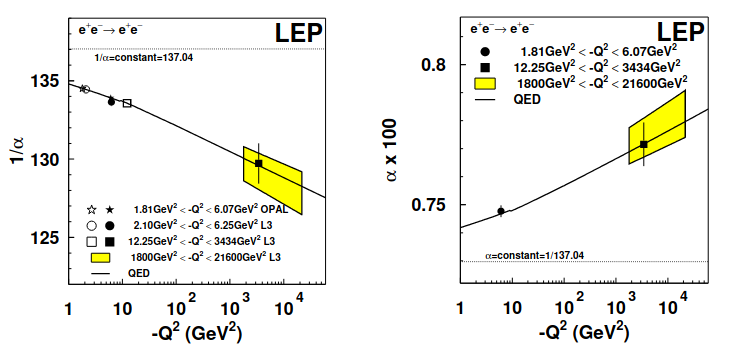
\includegraphics[scale=0.5]{chapter1/alphas1.png}
\caption{Trend of QED running coupling constant with $Q^{2}$~(left), QCD running coupling constant with $Q^{2}$~(right),~figure adopted from~\cite{ACHARD200526}.}
\end{figure}
\begin{figure}[h!]
\centering
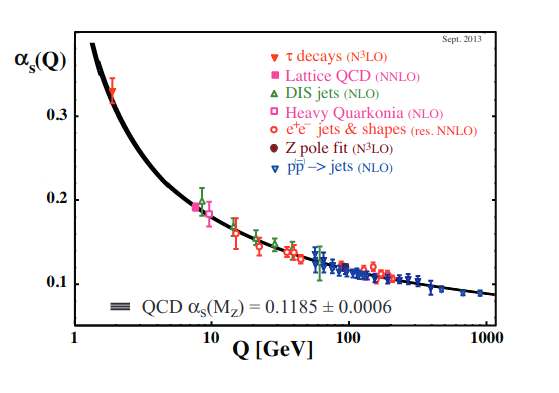
\includegraphics[scale=0.6]{chapter1/alphs1.png}
\caption{The change in the vale of $\alpha_{S}$ with the energy scale Q and the current world average value is illustrated,~Figure taken from~\cite{denterria2015highprecision}}
\end{figure}

\subsection{Theory of Weak Interactions}
Weak interaction are mediated by (as photons for QED and gluons for QCD) the $W$ and $Z^{0}$ bosons and these mediators are extremely heavy. Experimentally $M_{w}=80.387~\pm~0.016~GeV$~\cite{PhysRevD.98.030001} and $M_{z}=91.188~\pm~0.0031~GeV$~\cite{PhysRevD.98.030001}.

We know that the massless photons and gluons have two polarization states after imposing Lorentz condition and Coulomb gauge condition but particles with mass and spin one, are allowed to have three polarization states~$m_{s}=(-1,0,1)$, Thus for the $W$ and $Z$ boson the completeness relation is quite different and propagator factor no longer remain same but becomes,$\frac{\iota g_{\mu\nu}}{Mc^{2}}$ here we assume $q^{2}<<(Mc^{2})$.
\subsubsection{Charged Weak Interaction}
\begin{center}
\feynmandiagram [vertical=a to b] {
i1 [particle=\(e(p1)\)] -- [fermion] a -- [fermion] i2 [particle=\(\nu_{e}p(3)\)],
a -- [boson, edge label=\(W\)] b,
f1 [particle=\(\mu p(4)\)] -- [anti fermion] b -- [anti fermion] f2 [particle=\(\nu_{\mu}p(2)\)],
};
\end{center}
Considered the process,
$\nu_{\mu}+e^{-}\rightarrow\mu^{-}+\nu_{e}$
The amplitude for this interaction is
\begin{equation}
\mathcal{M}=\frac{g_{W}^{2}}{8(M_{w}c^{2})}[\overline{u}(3)\gamma^{\mu}(1-\gamma^{5})u(1)][\overline{u}(4)\gamma_{\mu}(1-\gamma^{5})u(2)],
\end{equation}
Here $\gamma^{\mu}$ alone represents vector coupling whereas $\gamma^{\mu}\gamma^{5}$ would be an axial vector. When we mix a vector to an axial vector then we are bound to violate the parity conservation, that is what happens in weak interactions. Here $g_{w}=\sqrt{4\pi\alpha_{w}}$ and its value is 0.653, and hence the weak fine structure constant is $\alpha_{w}=\frac{1}{29.5}$. This coupling constant is roughly 5 times larger than that of QED but weak interaction are feeble because of massive mediators $W$ and $Z$ bosons.

\subsubsection{Decay of Neutron}
\begin{center}
\feynmandiagram [vertical=a to b] {
i1 [particle=\(n(p1)\)] -- [fermion] a -- [fermion] i2 [particle=\(p(p3)\)],
a -- [boson, edge label=\(W\)] b,
f1 [particle=\(e(p4)\)] -- [anti fermion] b -- [fermion] f2 [particle=\(\nu_{e}(p2)\)],
};
\end{center}

The above Feynman diagram shows the beta decay of neutron, by applying Feynman calculus we find that the neutron life time $\tau=\frac{1}{\Gamma}=1318~s$, as the experimental neutron lifetime is $885.7\pm0.8$~\cite{serebrov2019neutron} seconds. The problem arises due to fact that we treat the proton and neutron as a point particles like leptons, which interact with the $W$ boson. We don't know, what kind of structure protons and neutrons have and what kind of interactions are going on inside proton~i.e.~(valence quarks interaction with gluon, quark pairs formed by gluons, hadronisation) but all  the finalized activity conserves charge. This problem arises becuse we don't know how quarks couple with the vector bosons.
\subsubsection{Neutral Weak Interaction}
\begin{center}
\feynmandiagram [vertical=a to b] {
i1 [particle=\(e(p1)\)] -- [fermion] a -- [fermion] i2 [particle=\(e(p3)\)],
a -- [boson, edge label=\(Z\)] b,
f1 [particle=\(\overline{\nu}_{\mu}(p4)\)] -- [fermion] b -- [fermion] f2 [particle=\(\overline{\nu}_{\mu}(p2)\)],
};
\end{center}

The above Feynman diagram shows $\overline{\nu_{\mu}}+e\rightarrow\overline{\nu_{\mu}}+e$ process mediated by $Z$ boson.
The vertex factor for the $Z^{0}$ boson is not so simple;
\begin{equation}
\frac{-\iota g_{z}}{2}\gamma^{\mu}(c_{v}^{f}-c_{A}^{f}\gamma^{5})
\end{equation}

Where $g_{z}$ is the neutral coupling constant, and the coefficient, $c_{v}^{f}$ and $c_{A}^{f}$ depend on the particular quark or lepton involved. All these parameters are determined by single parameter called $\theta_{W}$ the 'weak mixing angle'. The weak and electromagnetic coupling constant are related:
\begin{equation}
g_{e}=\frac{g_{e}}{sin\theta_{w}},    g_{z}=\frac{g_{e}}{sin_{\theta_{w}}cos_{\theta_{w}}}
\end{equation}
The experimental value of $\theta_{w}$ is 28.75. The amplitude for the above scattering at low energies~($q^{2}<<M_{z}^{2}c^{2}$) is:
\begin{equation}
\mathcal{M}=\frac{g_{z}^2}{8(M_{Z}c)^2}[\overline{u}(3)\gamma^{\mu}(1-\gamma^{5})u(1)][\overline{u}(4)\gamma_{\mu}(c_{v}-c_{A}\gamma^{5})u(2)]
\end{equation}\\

\section{Gauge Symmetry}
The lagrangian densities for the fermionic and electromagnetic fields can be written~\cite{Quarks&lepton87}\\
K-G equation:
\begin{equation}
\mathcal{L}=\frac{1}{2}(\partial_{\mu}\phi)(\partial^{\mu}\phi)-\frac{1}{2}m^{2}\phi^{2},
\end{equation}
Dirac equation:
\begin{equation}
\mathcal{L}=\iota\overline{\psi}\gamma^{\mu}\partial_{\mu}\psi-m\overline{\psi}\psi,
\end{equation}
Maxwell equation:
\begin{equation}
\mathcal{L}=\frac{-1}{4}F^{\mu\nu}F_{\mu\nu}-j^{\mu}A_{\mu},
\end{equation}

Now if we transform the field $\psi$ of the Dirac Lagrangian as $\psi\rightarrow\psi^{\prime}=e^{\iota\alpha}\psi$ where $\alpha$ is some constant. Such transformation of field is called Global gauge transformation and Lagrangian $\mathcal{L}$ remains invariant under such transformation.
To make the Lagrangian invariant under local gauge transformation $\psi\rightarrow\psi^{\prime}=e^{\iota\alpha(x)}\psi$ we have to introduce an extra term in the Dirac Lagrangian which corresponds to electromagnetic interaction and the Lagrangian becomes:
\begin{equation}
\mathcal{L}=\iota\overline{\psi}\gamma^{\mu}\partial_{\mu}\psi-m\overline{\psi}\psi+\frac{-1}{4}F_{\mu\nu}F^{\mu\nu}-j^{\mu}A_{\mu},
\end{equation}


\subsubsection{Higgs Mechanism and Higgs Boson}

The electromagnetic and weak force can be described with the same theory, thus with this unification we can say that electromagnetic and weak forces can be treated as a single force known as the electroweak force.

The unification theory correctly explains the electromagnetic and weak field and associated force carrying particles but the problem is, according to this theory all the mediators are massless but $W$ and $Z$ bosons have mass up to  100 times of mass of proton. The theory which solve this puzzle is called Higgs mechanism. Which says that $W$ and $Z$ bosons acquire mass with the interaction of invisible field called Higgs field.

To understand the electroweak interaction we have to construct Lagrangian that is invariant under the $SU(2)\times U(1)$ transformation.
But we know that $W$ and $Z$ bosons are massive and with the mass term in Electro-weak Lagrangian we must break the gauge invariance. We can write the Lagrangian for weak interaction~\footnote{For detail see chapter 14 of Quarks and Lepton: An introductory course in Modern physics by Francis Halzen Alan D.Martin}:
\begin{equation}
\mathcal{L}=\overline{\psi}\iota\gamma^{\mu}\partial_{\mu}\psi+\iota\frac{f}{2}\tau.W_{\mu}\psi-\frac{1}{4}W_{\mu\nu}W^{\mu\nu},
\end{equation}
here the last term corresponds to weak field tensor.

But we need mass for the $W$ and $Z$ boson and with the mass term Lagrangian is no more gauge invariant, so we have to break the gauge symmetry. So together with mass term in Lagrangian along with gauge symmetry we introduce a Lagrangian:
\begin{equation}
\mathcal{L}=\frac{-1}{4}B_{\mu\nu}B^{\mu\nu},
\end{equation}
where $B_{\mu\nu}=\partial_{\mu}B^{\mu}-\partial_{\nu}B^{\mu}$ and it transforms like $A^{\mu}$
\begin{equation}
B^{\mu}\rightarrow B^{\prime}{\mu}=B^{\mu}+\partial^{\mu}\Lambda,
\end{equation}
where $\Lambda$ is some scalar function and $B^{\mu}$ is some vector field. The Lagrangian becomes:
\begin{equation}
\mathcal{L}=\frac{-1}{4}B_{\mu\nu}B^{\mu\nu}+\mathcal{L}_{scaler},
\end{equation}
\begin{equation}
\mathcal{L}_{scaler}=(D_{\mu}\phi)^{*}(D^{\mu}\phi)-V(\phi^{*}\phi),
\end{equation}

\begin{equation}
D_{\mu}=\partial^{\mu}-\iota gB^{\mu},
\end{equation}
and $\phi$ is some complex field given by $\phi(x)=e^{\iota\phi(x)}(\frac{v+h(x)}{\sqrt{2}})$,and $B^{\mu}\rightarrow B^{\prime\mu}=B^{\mu}+\frac{1}{g}.\partial^{\mu}\theta$ Now  If we make a gauge transformation
\begin{equation}
\phi\rightarrow\phi^{\prime}=e^{i\theta}.\phi,
\end{equation}
\begin{equation}
B_{\mu}\rightarrow B_{\mu}^{\prime}=B_{\mu}+\frac{1}{g}\partial^{\mu}\theta,
\end{equation}
we also have a mass term in the Lagrangian which can be written as:
\begin{equation}
M_{B}=\frac{g^{2}v^{2}}{2},
\end{equation}
and energy term:
\begin{equation}
V=\lambda(\phi^{*}\phi-\frac{v^{2}}{2})^{2},
\end{equation}
thus for minimum energy of scalar field $\phi$ by setting $\frac{\partial v}{\partial \phi}=0$ we get:
\begin{equation}
<\phi>=\begin{pmatrix}
0\\
\frac{V}{\sqrt{2}}
\end{pmatrix}
\end{equation}


corresponds to vacuum. This means when we say vacuum we don't have presence of physical particles or physical fields. Then quantum fluctuation or particles can be created by  giving energy greater than $<\phi>$. Thus presence of $<\phi>$~(Higgs field) gives the mass $M_{B}$ through the interaction of $B_{\mu}$ field with $\phi$ Higgs field.
\begin{figure}[h!]
\begin{tabular}{cc}
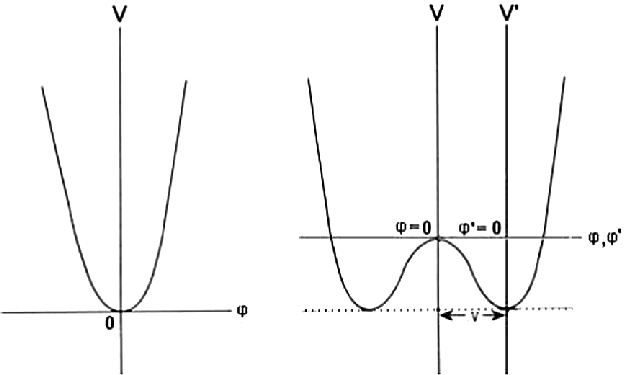
\includegraphics[scale=0.3]{chapter1/Symmetry breaking.png}
&
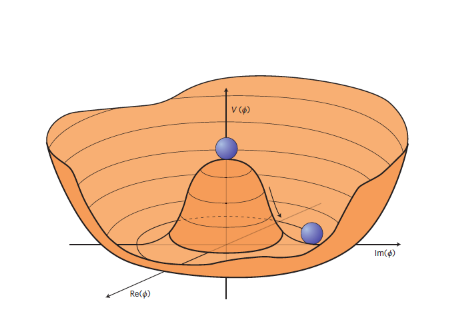
\includegraphics[scale=0.5]{chapter1/sym_break.png}
\end{tabular}

\caption{The potential V of a complex scaler field $\phi$~\cite{Ellis_2016}}
\end{figure}
The physical particles that corresponds to $\phi$ are $h$ 'Higgs Boson'. The vacuum potential configuration does not have $\phi = 0$ state and the field is said to have a non-zero vacuum expectation value $v$, Due to symmetric configuration of vacuum potential there will be two degenerate states, any vacuum state of the field will have $\phi$ = +v or $\phi$ = -v value. Thus the choice of any vacuum state breaks the symmetry of the Lagrangian, also called \textit{spontaneous symmetry breaking}.
The masses for the vector bosons can be expressed in terms of $\nu$ and the electroweak coupling constant g:
\begin{equation}
\begin{tabular}{cc}
$m_{W}=\frac{1}{2}\nu g
$&$
m_{Z}=\frac{m_{w}}{cos\theta_{W}}=\frac{1}{2}\nu\sqrt{g^{2}+g\prime^{2}}
$
\end{tabular}
\end{equation}
Where $\theta_{W}$ is defined by:
\begin{equation}
tan\theta_{W}\equiv \frac{g^{\prime}}{g}\longrightarrow sin^{2}\theta_{W}=1-\frac{m_{W}^{2}}{m_{Z}^{2}},
\end{equation}

\section{Hadron Collider Physics}
Hadrons are the bound colourless states of quarks confined by gluon interactions, of which the proton is a stable example. Collisions in high energy experiments result in the ‘hard’ or high-$Q^{2}$ scattering of accelerated particles dominating interactions between composite particles, which produce additional soft-QCD processes. This results in a perturbative high energy process and a non-perturbative low energy background present in proton-proton collisions.\\
In hadron collision experiments at a sufficiently high momentum transfer, one can approximate all partons as free particles. Thus hadron-hadron interaction can be thought of as single parton-parton interaction.~\cite{Mead:2780780}. The parton momentum can be expressed in terms of the fraction of the hadron momentum $p_{parton}=x.p_{hadron}$, where $x$ is also referred as "Bjorken scaling variable". Then, the probability of finding two parton flavors $f_{I}$ with momentum fraction $x_{i}$ interacting at an energy scale $\mu_{F}$
in a hadron-hadron collision is given by the parton distribution function (PDF) as PDF$(x_{1},f_{1}\mu_{F})$ and PDF$(x_{2},f_{2},\mu_{F})$ which will be discussed in detail in chapter~3.

In other words, at sufficiently high energies, interactions between the constituents of a proton are neglected. This allows factorisation of the perturbative calculable partonic cross section from that of the overall interaction, assuming asymptotic freedom for each possible set of initial states. Each contribution is weighted by the relevant parton distribution functions (PDFs), which act as the parameterisation of the contents of hadrons in the collisions taking place.
\begin{equation}
\sigma_{AB\rightarrow x}=\int dx_{A}dx_{B}f_{a}(x_{a},\mu_{F},\mu_{R})f_{b}(x_{b},\mu_{F},\mu_{R})\sigma_{ab}\rightarrow x
\end{equation}
The factorisation theorem provides the hadronic cross section in these terms, where $A$ and $B$ are the colliding hadrons, $a$ and $b$ are the scattered partons and $f_{a}(x_{a},Q^{2})$, $f_{b}(x_{b},Q^{2})$ are the PDFs for parton $a$ and $b$. The partonic cross section depend upon $\alpha_{s}(\mu_{R}^{2})$, where $\mu_{R}$ and $\mu_{F}$ are the re-normalisation and factorisation scale and $x$ is independent of the number of final state particles or kinematic configuration.


